\documentclass[11pt,a4paper,twoside]{article}
\usepackage[utf8]{inputenc}
\usepackage[T1]{fontenc}

\usepackage{mathptmx}
\usepackage{datetime}
\usepackage[spanish, es-nolists]{babel}
\usepackage{amsmath}
\usepackage{amsthm}
\usepackage{amsfonts}
\usepackage{amssymb}
\usepackage{titlesec}
\usepackage{graphicx}
\usepackage{mathtools}

\decimalpoint

\usepackage{array}
\usepackage{float}
\usepackage[a4paper]{geometry}
\geometry{top=2.5cm, bottom=2cm, left=2.54cm, right=2.54cm}
\usepackage{fancyhdr}
\pagestyle{fancy}
\fancyhf{}  % Limpiar los encabezados y pies de página predeterminados
% Encabezados para páginas impares
\fancyhead[LE,RO]{\thepage} % En la izquierda de la página impar
\fancyhead[RE]{\textsc{Anónimo}} % En la derecha de la página impar
% Encabezados para páginas pares
\fancyhead[LO]{\textit{Generación y optimización de código}}  % En la izquierda de la página par
\fancyfoot{}

\usepackage{color}
\usepackage{cancel}
\usepackage{ulem}
\usepackage{tcolorbox}
\usepackage{multirow}
\usepackage{tikz}
\usetikzlibrary{babel, arrows.meta, arrows, datavisualization, patterns}
\usepackage{multicol}
\usepackage{stackrel}
\usepackage{pdfpages}
\renewcommand{\labelitemi}{\textbullet}

\theoremstyle{definition}
\newtheorem{ejemplo}{\textbf{Exemplo}}
\newtheorem{ejer}{\textcolor{red}{\textbf{Exercicio}}}
\newtheorem{defi}{\textbf{Definición}}
\newtheorem{theorem}{\textbf{Teorema}}
\newtheorem{lema}{\textbf{Lema}}
\newtheorem{corol}{\textbf{Corolario}}
\newtheorem{prop}{\textbf{Proposición}}
\newtheorem{nota}{\textbf{\textit{Nota}}}

\renewcommand\qedsymbol{$\blacksquare$}

\usepackage{hyperref}
\hypersetup{
	colorlinks,
	citecolor=black,
	filecolor=black,
	linkcolor=black,
	urlcolor=black
}

\usepackage{enumitem}


\newcommand{\imagen}[1]{
	\begin{figure} [H] \centering
		\includegraphics[width=\textwidth]{#1}
	\end{figure}
}

\title{%
	\LARGE \textbf{Compiladores e Intérpretes} \\ \vspace*{1cm} \textbf{Práctica 2: Generación y optimización de código}
	\\ \Large \textbf{Reemplazo de multiplicaciones y divisiones enteras por operaciones de desplazamiento}}
\author{\textsc{Autor anónimo}}
\date{Universidade de Santiago de Compostela}

\setlength{\parskip}{5pt}

\usepackage{setspace}

\onehalfspacing % Configura el interlineado a 1.5

\setlength{\parindent}{0.7cm}

\usepackage[hang, small,labelfont=bf,up,textfont=up]{caption}
\usepackage{hanging}
\usepackage{sectsty}

\sectionfont{\fontsize{14}{15}\selectfont}
\subsectionfont{\fontsize{12}{15}\selectfont}
\subsubsectionfont{\fontsize{12}{15}\selectfont}

\usepackage{titlesec}
\titleformat{\subsection}[block]{\normalfont\large\itshape}{\thesubsection}{1em}{}
\titlespacing*{\section}
{0pt}{\baselineskip}{0pt}
\titlespacing*{\subsection}
{0pt}{\baselineskip}{0pt}
\titlespacing*{\subsubsection}
{0pt}{\baselineskip}{0pt}

\usepackage[cache=false]{minted}
\definecolor{bg}{rgb}{.95, .95, .95}

\usepackage[backend=biber, style=ieee, sorting=nty]{biblatex}
\bibliography{references}


\begin{document}
	
	% PORTADA
	\maketitle
	\thispagestyle{empty}
	
	\vspace*{1cm}
	
	% ÍNDICE
	\renewcommand{\contentsname}{Índice} % Cambia el título
	\tableofcontents


	\newpage


	\section{Introducción}
	
	El rendimiento de los programas informáticos depende en gran medida de cómo se implementen las operaciones aritméticas, especialmente en bucles intensivos en cálculos. En esta práctica se analiza una técnica clásica de optimización a bajo nivel: el reemplazo de multiplicaciones y divisiones enteras por potencias de dos mediante operaciones de desplazamiento binario. Esta transformación permite, en muchos casos, reducir el coste computacional asociado a estas operaciones, aprovechando que los desplazamientos ($\ll$, $\gg$) se ejecutan generalmente más rápido que las multiplicaciones o divisiones en la mayoría de arquitecturas modernas.
	
	El objetivo principal del estudio es implementar dicha optimización sobre el código proporcionado, evaluar su impacto en el rendimiento y analizar su escalabilidad con respecto al tamaño del problema y al número de repeticiones (\texttt{ITER}). Para obtener medidas fiables, se realizan múltiples ejecuciones de cada versión del código (con y sin optimización), compiladas con el nivel de optimización \texttt{-O0} para evitar interferencias de otras transformaciones automáticas del compilador. Asimismo, se analiza el código ensamblador generado con el fin de confirmar que la sustitución ha tenido efecto y para entender mejor las diferencias observadas en los tiempos de ejecución.
	
	La práctica se completa con una interpretación de los resultados experimentales y un estudio de cómo influyen factores como la memoria caché y el número de repeticiones sobre la estabilidad y precisión de las medidas de tiempo, aportando una visión más completa sobre los beneficios reales de aplicar esta optimización.
	

	\section{Descripción de la técnica}

	El desplazamiento de bits es una operación que consiste en mover los bits de un número binario hacia la izquierda o hacia la derecha una cantidad determinada de posiciones. Esta técnica es fundamental en programación de bajo nivel y se utiliza con frecuencia en ámbitos como sistemas embebidos, procesamiento gráfico y optimización de rendimiento, ya que permite realizar operaciones rápidas y con control detallado a nivel de bits, según se explica en \cite{burrell}.
	
	Una operación de \textbf{desplazamiento a la izquierda} ($\ll$) mueve todos los bits de un número binario hacia la izquierda, rellenando con ceros los bits vacíos del lado derecho. Esta operación equivale a multiplicar el número original por $2^n$, donde $n$ es el número de posiciones desplazadas. Por ejemplo, desplazar un número una posición a la izquierda es equivalente a multiplicarlo por 2.
	
	De forma análoga, una operación de \textbf{desplazamiento a la derecha} ($\gg$) traslada los bits hacia la derecha. Si el desplazamiento es {lógico}, los bits vacíos del lado izquierdo se rellenan con ceros; si es {aritmético}, se conserva el bit de signo en números con representación en complemento a dos. Esta operación es equivalente, en muchos casos, a una división entera por potencias de dos.
	
	El uso de desplazamientos puede reemplazar multiplicaciones o divisiones enteras por potencias de dos, lo que permite reducir el coste computacional de estas operaciones en ciertas arquitecturas. Esto puede dar lugar a algoritmos más rápidos y eficientes, especialmente en aplicaciones críticas para el rendimiento, como el procesamiento gráfico, la criptografía o la indexación de grandes volúmenes de datos.
	
	El código con multiplicaciones y divisiones inicialmente propuesto es:
	\begin{minted}[linenos,fontsize=\small,
		bgcolor=bg]{c}
int i, j, m3 = 8, m5 = 32, a = 0, b = 0;
for (j = 0; j < ITER; j++) {
	for (i = 0; i < N; i++) {
		a = i * m3;
		b += a / m5;
	}
}
	\end{minted}

	Es claro que \texttt{a} representa el valor del índice (sobre el tamaño del problema) multiplicado por $2^3=8$, para luego sumar de forma acumulada \texttt{b} con \texttt{a} dividido entre $2^5=32$.

	La optimización que se implementará será la siguiente. Un simple análisis llega para ver que:
	\begin{equation}\label{eq:uno}
		\texttt{b} = \texttt{b} + \dfrac{\texttt{a}}{2^5} = \texttt{b} + \dfrac{i \cdot 2^3}{2^5} = \texttt{b} + \dfrac{i}{2^2}.
	\end{equation}
	
	En la versión optimizada del código tenemos en cuenta (\ref{eq:uno}) e implementamos la operación con un desplazamiento de 2 bits a la derecha, como se ha explicado.
	\begin{minted}[linenos,fontsize=\small,
		bgcolor=bg]{c}
for (j = 0; j < ITER; j++) {
	for (i = 0; i < N; i++) {
		b += i >> 2;
	}
	a = (N - 1) << 3;
}
	\end{minted}

	De manera similar, para intentar ser fiel con el cálculo de \texttt{a} en cada uno de los índices sobre \texttt{ITER}, terminamos la iteración multiplicando como sigue. El término $\texttt{a}_i$ se refiere al valor de \texttt{a} antes de comenzar la iteración $i+1$ sobre \texttt{ITER}.
	\begin{equation}\label{eq:dos}
		\forall i, \:\: \texttt{a}_i = i \cdot 2^3 \implies \texttt{a}_{N-1} = (N-1)\cdot 2^3.
	\end{equation}
	
	Además de su uso en operaciones aritméticas, el desplazamiento de bits permite manipular directamente bits individuales, lo cual resulta útil para configurar, borrar o alternar banderas dentro de registros binarios. Comprender estas operaciones es esencial para aquellos que deseen profundizar en el funcionamiento interno del \textit{hardware} y en la eficiencia del software a bajo nivel.
	
	Para ambas versiones, se explica a continuación la motivación de los 2 bucles anidados.
	
	\subsection{Configuración del experimento}
	
	El objetivo del experimento es analizar el comportamiento de la versión con multiplicaciones y divisiones frente a la versión con operaciones de desplazamiento para diversos tamaños del problema. Para esto, se crea un \textit{array} de valores de \texttt{N} con un número de datos suficiente (40 valores diferentes) y evitando potencias enteras de 2. El \textit{array} se muestra en (\ref{eq:n}).
	
	\begin{equation}\label{eq:n}
		\begin{aligned}
			\texttt{N} = \left(
			\begin{matrix}
				3000,      & 4500,      & 7000,      & 9500,      & 12000,		\\
				17000,     & 25000,     & 34000,     & 40000,     & 56000,		\\
				78000,     & 95000,     & 110000,    & 160000,    & 250000,		\\
				320000,    & 390000,    & 570000,    & 820000,    & 1000000,	\\
				1190000,   & 1500000,   & 1750000,   & 1990000,   & 2550000,	\\ 
				3190000,   & 4200000,   & 5100000,   & 5900000,   & 7800000,	\\
				9500000,   & 11800000,  & 15900000,  & 23900000,  & 53000000,	\\
				95000000,  & 199000000, & 383000000, & 959000000, & 1910000000	\\
			\end{matrix}
			\right).
		\end{aligned}
	\end{equation}

	Además, resulta importante incluir un bucle externo de número fijo de iteraciones (\texttt{ITER}) cuando se estudia el rendimiento de un algoritmo en función del tamaño del problema, especialmente si este es variable, para garantizar condiciones comparables entre ejecuciones con distintos valores de N. Para valores pequeños de \texttt{N}, la ejecución del algoritmo es demasiado rápida. Esto puede provocar medidas ruidosas y poco precisas por debajo del umbral de resolución del reloj del sistema, aparte de un dominio del \textit{overhead} de la llamada al sistema o del propio cronómetro (si este no valiese 0).
	
	Sin embargo, para valores grandes de tamaño del problema, el algoritmo tarda más, pero con mucha menor variabilidad relativa. Esto genera datos incomparables y gráficas sesgadas. Se introduce así un bucle externo de \texttt{ITER} repeticiones, donde \texttt{ITER} se elige dinámicamente para que el producto $\texttt{ITER} \cdot \texttt{N}$ sea constante (o aproximadamente constante). Fijando que cada repetición del experimento deba tardar, al menos, una decena de segundos, generamos el vector de \texttt{ITER} según (\ref{eq:ITER}), que garantiza esta condición.
	
	\begin{equation} \label{eq:ITER}
		\forall i \in \lbrace 1, \dots, 40 \rbrace, \:\: \texttt{ITER}_i = \left\lfloor \dfrac{6.400.000.000}{\texttt{N}_i} \right\rfloor.
	\end{equation}

	Esta expresión se traducirá en el código C en la función \texttt{generar\_iter()}. Para el vector (\ref{eq:n}), los valores corrrespondientes se reflejan en (\ref{eq:ejITER}).
	
	\begin{equation} \label{eq:ejITER}
		\begin{aligned}
			\texttt{ITER} = \left(
			\begin{matrix}
				2133333, & 1422222, & 914285, & 673684, & 533333, \\
				376470, & 256000, & 188235, & 160000, & 114285, \\
				82051, & 67368, & 58181, & 40000, & 25600, \\
				20000, & 16410, & 11228, & 7804, & 6400, \\
				5378, & 4266, & 3657, & 3216, & 2509, \\
				2006, & 1523, & 1254, & 1084, & 820, \\
				673, & 542, & 402, & 267, & 120, \\
				67, & 32, & 16, & 6, & 3 \\
			\end{matrix}
			\right).
		\end{aligned}
	\end{equation}

	Para cada valor de \texttt{N}, es fundamental ejecutar el algoritmo un número suficiente de veces, denotado como \texttt{REPETICIONES}, con el fin de obtener medidas de rendimiento representativas y estables. La variabilidad inherente al sistema ---debido a factores como la planificación del sistema operativo, el estado de la caché, o procesos en segundo plano--- puede provocar fluctuaciones significativas en los tiempos de ejecución individuales. Al repetir las mediciones y calcular posteriormente estadísticas como la \textbf{media}, el \textbf{máximo} y el \textbf{mínimo}, se obtiene una caracterización más completa del comportamiento del algoritmo. Estas métricas permiten representar en las gráficas no solo la tendencia central, sino también la dispersión y los extremos del rendimiento, ofreciendo una visión más realista y robusta para comparar implementaciones o analizar cuellos de botella. Para este particular, \texttt{REPETICIONES} se fija a 20.
		
	
	\section{Beneficios y desventajas esperados}
	
	Las técnicas de \textbf{reducción por fuerza}, como se ve en \cite{aho} (sección 8.7.4), permiten reemplazar operaciones costosas por otras equivalentes pero más eficientes en la máquina objetivo. Estas transformaciones están motivadas por el hecho de que ciertas instrucciones del conjunto de la arquitectura son mucho más económicas que otras. Por ejemplo, elevar un número al cuadrado, $x^2$, puede reemplazarse por la multiplicación $x \times x$, que resulta menos costosa que una llamada a una rutina de exponenciación general.
	
	Estas transformaciones, conocidas como reducción por fuerza local, se complementan con otras optimizaciones como la eliminación de operaciones redundantes mediante identidades aritméticas básicas y el plegado de constantes, contribuyendo todas a una generación de código más eficiente, según \cite{aho} (sección 8.5.4).
	
	Un caso particularmente interesante es el uso de \textbf{desplazamientos binarios} ($\ll$, $\gg$) como sustitutos de multiplicaciones o divisiones por potencias de dos. Estas operaciones, en principio, deberían ser más rápidas que una multiplicación o división convencional, ya que el \textit{hardware} puede implementarlas mediante simples circuitos de cableado sin necesidad de utilizar una unidad aritmética compleja.
	
	Sin embargo, en la práctica, esta ventaja no siempre se manifiesta de forma significativa. En arquitecturas modernas, las unidades aritméticas están tan optimizadas que las diferencias de coste entre una multiplicación por una constante y un desplazamiento pueden ser mínimas o incluso inexistentes, especialmente cuando el compilador ya realiza estas optimizaciones automáticamente, \textit{aún compilando sin optimizaciones}. Además, el uso de desplazamientos puede introducir ambigüedad o dificultar la legibilidad del código fuente si no se utiliza con criterio.
	
	De acuerdo a \cite{gcc}, la compilación en GCC con \texttt{-O0} reduce el tiempo de compilación y permite que la depuración produzca los resultados esperados. Este es el nivel predeterminado. Con la opción \texttt{-O0}, GCC desactiva completamente la mayoría de las pasadas de optimización; estas no se ejecutan ni siquiera si se habilitan explícitamente en la línea de comandos o si aparecen listadas como activadas por defecto.
	
	Por lo tanto, aunque los desplazamientos siguen siendo una herramienta útil en la optimización de bajo nivel ---especialmente en sistemas embebidos o compiladores de alto rendimiento---, es importante evaluar su beneficio real en el contexto específico de la arquitectura y el compilador utilizados.
	
	
	\section{Programación y código en ensamblador}
	
	\subsection{Arquitectura de compilación y ejecución}
	
	La compilación con la opción \texttt{-S} de GCC produce códigos fuente del ensamblador de la máquina mediante los que podemos analizar la traducción de las 2 estrategias. Se han ejecutado los códigos en una máquina ASUS Zenbook UX425EA 1.0, equipada con el sistema operativo Ubuntu 22.04.3 LTS x86\_64. Cuenta con un procesador Intel i7-1165G7 de 4 núcleos físicos de undécima generación, que funciona a una frecuencia de reloj de 2.80 GHz. Las direcciones de memoria ocupan 39 bits físicos y 48 bits virtuales.
	
	Cada núcleo dispone de 2 hilos de procesamiento, resultando en un total de 8 hilos. Dispone de 16 GiB de memoria RAM totales y de 4 niveles de memoria caché: L1d (192 KiB, 4 instancias), L1i (128 KiB, 4 instancias), L2 (5 MiB, 4 instancias) y L3 (12 MiB, 1 instancia). El TDP (\textit{Thermal Design Power}) es configurable entre 12 y 28 W. Se omite la inclusión de otros componentes como la tarjeta gráfica o de sonido porque no afectarán a los resultados de las pruebas. La versión del compilador utilizada es GCC 11.4.0.

	Con el fin de ejecutar las dos versiones en las mismas condiciones, se ha envuelto en cada caso el algoritmo en una estructura de bucles bajo \texttt{REPETICIONES} y variables de la forma que sigue:
	
	\begin{minted}[linenos, fontsize=\small, bgcolor=bg]{c}
int main() {
	int ITER[TAM_N]; // Array ITER del mismo tamaño que N
	generar_ITER(ITER); // Generar valores
	
	// Abrimos en modo escritura
	FILE *file = fopen(nombre_archivo, "w"); 
	if (!file) { ... }
	
	// Escribimos la cabecera en el archivo
	fprintf(file, "N\t ... \n");
	
	// No hay que calentar la caché porque no se usa ningún vector
	// solo se utilizan 3 variables que estarán en la pila
	
	// Medir overhead, que ha resultado 0, luego se obvia
	gettimeofday(&overhead_start, NULL);
	gettimeofday(&overhead_end, NULL);
	overhead = (overhead_end.tv_sec - overhead_start.tv_sec) +
	(overhead_end.tv_usec - overhead_start.tv_usec) / 1e6;
	
	// Variables locales
	int i, j, a = 0, b = 0; // y m3, m5
	
	for (int index = INDEX_INICIO; index < INDEX_FIN; index++) {
		double tiempos[REPETICIONES];
		int N_local = N[index], ITER_local = ITER[index];
		
		for (int k = 0; k < REPETICIONES; k++) {
			b=0;
			gettimeofday(&start_time, NULL);
			// algoritmo
			gettimeofday(&end_time, NULL);
			tiempos[k] = ((end_time.tv_sec - start_time.tv_sec +
			(end_time.tv_usec - start_time.tv_usec)/1.e6)
			- overhead)/ITER_local;
			fprintf(file, "%d\t%.6f\n", N_local, tiempos[k]);
		}
	}
	
	fclose(file);
	return 0;
}
	\end{minted}

	Los bloques denotados por el comentario \texttt{algoritmo} son los que se han descrito en la sección 2. En las dos versiones, el bucle externo de \texttt{ITER} se traduce en la directiva \texttt{.L10} y el bucle interno sobre \texttt{N} en \texttt{.L11}. El resto de instrucciones, puesto que se programa para ello, se traducen de forma idénticamente literal en el código ensamblador.

	\subsection{Bucles}
	
	En el caso de la versión original, los dos bucles explicados en la sección 2 se traducen en lo siguiente.
	
	\begin{minted}[linenos, fontsize=\small, bgcolor=bg]{nasm}
.L11:
	movl	-384(%rbp), %eax
	imull	-364(%rbp), %eax
	movl	%eax, -356(%rbp)
	movl	-356(%rbp), %eax
	cltd
	idivl	-360(%rbp)
	addl	%eax, -376(%rbp)
	addl	$1, -384(%rbp)
.L10:
	movl	-384(%rbp), %eax
	cmpl	-352(%rbp), %eax
	jl	  .L11
	addl	$1, -380(%rbp)
	\end{minted}

	Las instrucciones \texttt{imull} e \texttt{idivl}, que se corresponden con \texttt{a = i * m3} y \texttt{b += a / m5}, respectivamente, representan multipliciaciones y divisiones explícitas en cada iteración sobre un valor de \texttt{N}. Estas 2, teóricamente, son operaciones con un coste alto, aunque se podría ver reducido en computadores modernos.
	
	Para la versión con desplazamientos, los dos bucles anteriores se traducen en lo siguiente.
	
	\begin{minted}[linenos, fontsize=\small, bgcolor=bg]{nasm}
.L11:
	movl	-376(%rbp), %eax
	sarl	$2, %eax
	addl	%eax, -368(%rbp)
	addl	$1, -376(%rbp)
.L10:
	movl	-376(%rbp), %eax
	cmpl	-352(%rbp), %eax
	jl	  .L11
	movl	-352(%rbp), %eax
	subl	$1, %eax
	sall	$3, %eax
	movl	%eax, -356(%rbp)
	addl	$1, -372(%rbp)
	\end{minted}

	Las instrucciones \texttt{sarl} y \texttt{sall}, que se corresponden con \texttt{i $\gg$ 2} y \texttt{(N-1) $\ll$ 3}, respectivamente, son operaciones de desplazamiento de bits. Por lo tanto, estas suelen tardar 1 ciclo en cada llamada, lo que las haría en principio más rápidas que las aritméticas de multiplicación y división. A pesar de todo, con \texttt{-O0} el compilador no elimina accesos redundantes a memoria, por lo que se podría anular esta ventaja.
	
	
	\section{Resultados obtenidos}
	
	Los experimentos se han realizado teniendo en cuenta los parámetros \texttt{N}, \texttt{ITER} y \texttt{REPETICIONES} explicados en la sección 2. Las fases del experimento también se han introducido en la sección 4. No se ha realizado ninguna fase de calentamiento de la caché, ya que no se utiliza ningún vector para las operaciones, únicamente variables almacenadas en la pila (\texttt{a}, \texttt{b} y \texttt{c}). Seguidamente, se obtiene el \textit{overhead}, medición que tiene como objetivo estimar el tiempo que tarda en ejecutarse la propia medición del tiempo. Esto se aproxima calculando el tiempo que se tarda en usar \texttt{gettimeofday()} dos veces seguidas. Con todo, el \textit{overhead} ha resultado ser nulo durante las pruebas.
	
	\subsection{Tiempos de ejecución}
	
	La Figura \ref{graf:tiempos} representa los resultados obtenidos directamente de la ejecución del experimento. Para una más sencilla visualización, se presentan los ejes en escala logarítmica y se representan como puntos las medias de tiempo para cada valor de \texttt{N}, junto con el intervalo comprendido entre la mínima y la máxima medición (aunque en la mayoría de casos tiene longitud casi despreciable).
	
	\begin{figure} [H] \centering
		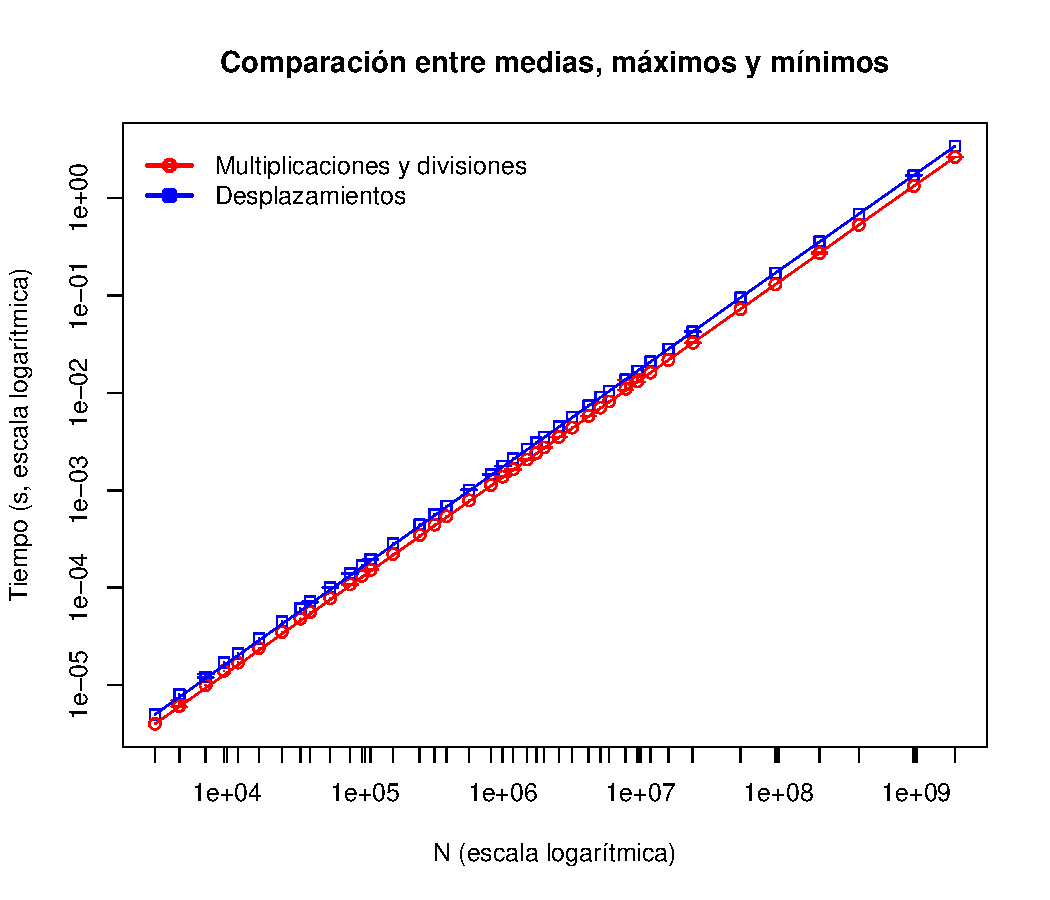
\includegraphics[width=.8\textwidth]{../graficas/NOCHE_tiempos.pdf}
		\caption{Comparativa global de los tiempos de ejecución.}
		\label{graf:tiempos}
	\end{figure}

	De forma aparentemente sorprendente respecto a lo desarrollado en la sección 3, la versión con multiplicaciones y divisiones enteras se ejecuta más rápido para todos los casos.
	
	\subsection{Aceleración}
	
	Una mejor manera de comparar las dos versiones del código es obtener la ganancia de una versión frente a la otra, es decir, la aceleración, que vendrá dada por:
	
	\begin{equation} \label{eq:speedup}
		ac = \dfrac{t_{\text{multiplicaciones, divisiones}}}{t_{\text{desplazamientos}}}.
	\end{equation}

	La Figura \ref{graf:speedup} implementa la expresión (\ref{eq:speedup}) tomando como referencia la media de tiempo de ejecución para cada \texttt{N}.
	
	\begin{figure} [H] \centering
		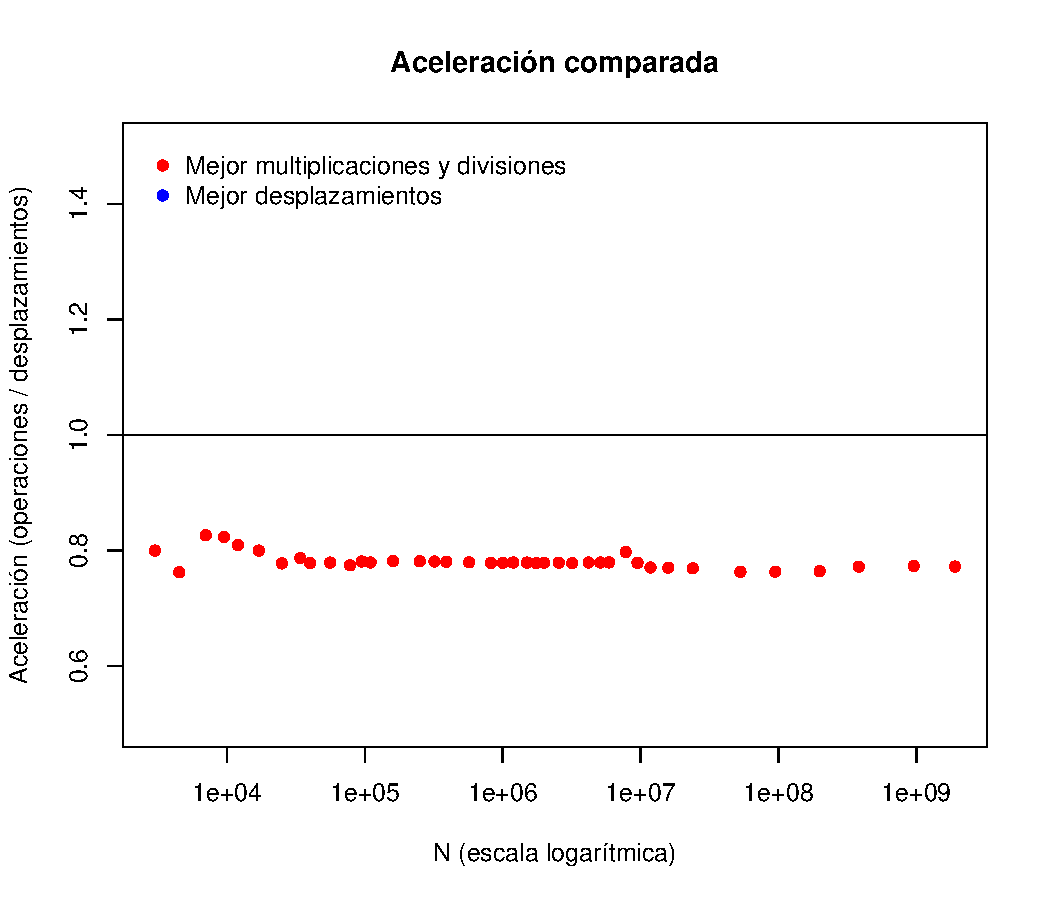
\includegraphics[width=.8\textwidth]{../graficas/NOCHE_speedup.pdf}
		\caption{Comparativa global de la aceleración media.}
		\label{graf:speedup}
	\end{figure}

	Viendo esta gráfica es ya claro que la versión que utiliza multiplicaciones y divisiones se ejecuta ligeramente más rápido que la que emplea desplazamientos.
	
	\subsection{Experimento reducido}
	
	Para intentar comprender por qué sucede lo anterior, pues contradice el punto de vista teórico, se ha desarrollado otro experimento a pequeña escala, que ha consistido en comparar la ejecución de múltiples veces en la misma máquina de una operación de multiplicación entre dos enteros que no son potencia entera de 2, una operación de multiplicación siendo uno de los enteros potencia entera de 2, y la misma operación de multiplicación implementada con un desplazamiento. Para la realización se han escogido diversos pares de la forma $(\texttt{N}_i, \texttt{ITER}_i)$ mostrados en (\ref{eq:n}) y (\ref{eq:ejITER}) y se ha repetido, en bucles anidados de igual manera, la operación correspondiente $\texttt{N}_i\cdot \texttt{ITER}_i$ veces.
	
	De forma análoga a lo ocurrido en el experimento principal, las versiones con multiplicación han ganado a la versión con desplazamientos en todos los casos. Por ejemplo, fijando operandos constantes $\texttt{a}=15$ y $\texttt{b}=33$ para la versión sin potencias enteras y $\texttt{a}=16$, con \texttt{b} idénticamente 33, y $\texttt{N}=95000$, los tiempos medios han sido los que aparecen en el Cuadro \ref{tabla1}.
	
	\begin{table} [H] \centering
		\begin{tabular} {| c | c | c |}
			\hline
			\textbf{Sin potencias de 2} & \textbf{Un operando es potencia de 2} & \textbf{Con desplazamientos} \\
			\hline
			 0.000142 & 0.000139 & 0.000162 \\
			 \hline
		\end{tabular}
		\caption{Ejemplo de comparativa de tiempos en el experimento reducido.}
		\label{tabla1}
	\end{table} 
	
	Esto sugiere que posiblemente el procesador ya efectúe optimizaciones en tiempo de ejecución (tales como paralelismo, reordenamiento de instrucciones, etc.) que no se pueden controlar de forma manual sobre las operaciones de multiplicación y división, reduciendo de forma efectiva el número de ciclos que tarda en realizarlas. Incluso es posible que el propio procesador haya implementado la instrucción de multiplicación como una secuencia de desplazamientos y sumas en código máquina.
	
	\section{Conclusiones}
	
	En el contexto de arquitecturas de CPU modernas, al menos en los experimentos realizados, no se han encontrado pruebas concluyentes que permitan afirmar que el uso de operaciones de desplazamiento (\textit{bit shift}) suponga una mejora en el tiempo de ejecución frente a multiplicaciones y divisiones enteras tradicionales. Esto se ha observado de forma consistente para cualquier valor correspondiente al tamaño del problema.
	
	En consecuencia, la optimización manual mediante desplazamientos no parece aportar ventajas de rendimiento generalizadas en este entorno, lo cual sugiere que los compiladores y procesadores actuales ya gestionan eficientemente este tipo de operaciones.


\printbibliography
	
	
	

\end{document}